% !TeX root = 系统动力学建模与仿真笔记.tex
% ============================================================
%  第七章 系统运动微分方程
% ============================================================

\section{系统动力学微分代数方程}

拉格朗日方程
\begin{equation}
    \frac{\mathrm{d}}{\mathrm{d}t}\left(\frac{\partial T}{\partial \dot{\bm{q}}}\right)^{\!\mathrm{T}}
    - \left(\frac{\partial T}{\partial \bm{q}}\right)^{\!\mathrm{T}}
    + \bm{\Phi}^{\mathrm{T}}\bm{\lambda} = \bm{Q}
    \label{eq:lagrange_dae}
\end{equation}
中，系统动能可表示为
\begin{equation*}
    T = \frac{1}{2}\dot{\bm{q}}^{\mathrm{T}}\bm{M}(\bm{q})\dot{\bm{q}},
\end{equation*}
式中 $\bm{M} = \bm{M}^{\mathrm{T}}$ 为对称矩阵。由此可得
\begin{align}
    \frac{\partial T}{\partial \dot{\bm{q}}} &= \dot{\bm{q}}^{\mathrm{T}}\bm{M}, \\[6pt]
    \frac{\mathrm{d}}{\mathrm{d}t}\left(\frac{\partial T}{\partial \dot{\bm{q}}}\right) &= \ddot{\bm{q}}^{\mathrm{T}}\bm{M} + \dot{\bm{q}}^{\mathrm{T}}\dot{\bm{M}}.
\end{align}
将上式代入拉格朗日方程~(\ref{eq:lagrange_dae})，可得系统运动微分方程
\begin{equation}
    \bm{M}\ddot{\bm{q}} + \dot{\bm{M}}\dot{\bm{q}} - \bm{T}_q^{\mathrm{T}} + \bm{\Phi}^{\mathrm{T}}\bm{\lambda} = \bm{Q}.
    \label{eq:eom_raw}
\end{equation}
系统运动微分方程~(\ref{eq:eom_raw})可表示为如下形式
\begin{equation}
    \boxed{\bm{M}\ddot{\bm{q}} + \bm{\Phi}^{\mathrm{T}}\bm{\lambda} = \bm{h}},
    \tag{I}
    \label{eq:eom_matrix}
\end{equation}
式中
\begin{equation}
    \bm{h} = \bm{Q} - \dot{\bm{M}}\dot{\bm{q}} + \bm{T}_q^{\mathrm{T}}.
    \label{eq:h_def}
\end{equation}

\begin{remark}
表达式~(\ref{eq:eom_matrix})中各矩阵与系统广义坐标 $\bm{q}$ 和广义速度 $\ddot{\bm{q}}$ 的关系满足
\[
    \bm{M}(\bm{q}(t)),\quad \bm{\Phi}(\bm{q}(t),t),\quad \bm{h}(\bm{q}(t),\dot{\bm{q}}(t),t).
\]
\end{remark}

对于一个完整系统，系统动力学方程由系统运动微分方程~(\ref{eq:eom_matrix})和几何约束代数方程构成，即
\begin{equation}
    \begin{cases}
        \bm{M}\ddot{\bm{q}} + \bm{c}_q^{\mathrm{T}}\bm{\lambda} = \bm{h}, & \text{(I)}\\[4pt]
        \bm{c}(\bm{q},t) = \bm{0}, & \text{(II)}
    \end{cases}
    \label{eq:DAE_system}
\end{equation}
这组微分代数方程 (Differential-Algebraic Equations, DAE) 的定解条件由初始时刻 ($t = t_0$) 的系统广义坐标和广义速度确定，即
\begin{equation*}
    \begin{cases}
        \bm{q}(t)\big|_{t=t_0} = \bm{q}_0,\\[4pt]
        \dot{\bm{q}}(t)\big|_{t=t_0} = \dot{\bm{q}}_0.
    \end{cases}
\end{equation*}
$\bm{q}_0$ 和 $\dot{\bm{q}}_0$ 同时满足位置级约束方程 (III) 和速度级约束方程 (IV)，即
\begin{equation}
    \begin{cases}
        \bm{c}(\bm{q}_0,t_0) = \bm{0}, & \text{(III)}\\[4pt]
        \bm{c}_q(\bm{q}_0,t_0)\dot{\bm{q}}_0 + \bm{c}_t(\bm{q}_0,t_0) = \bm{0}. & \text{(IV)}
    \end{cases}
    \label{eq:initial_conditions}
\end{equation}

\section{习题}

\paragraph{习题说明}

针对后文描述的在惯性坐标系 $OXY$ 平面内运动的动力学系统及选定的广义坐标 $\bm{q}$，列写如下矩阵形式的系统运动微分方程
\begin{equation*}
    \begin{bmatrix}
        \bm{M} & \bm{c}_q^{\mathrm{T}}\\[3pt]
        \bm{c}_q & \bm{O}
    \end{bmatrix}
    \begin{bmatrix}
        \ddot{\bm{q}}\\[3pt]
        \bm{\lambda}
    \end{bmatrix}
    =
    \begin{bmatrix}
        \bm{h}\\[3pt]
        \bm{\varepsilon}
    \end{bmatrix},
\end{equation*}
并给出系统运动微分方程中
\[
    \bm{M}(\bm{q}),\quad \bm{c}_q(\bm{q}),\quad \bm{h}(\bm{q},\dot{\bm{q}},t),\quad \bm{\varepsilon}(\bm{q},\dot{\bm{q}},t)
\]
的具体表达式。重力加速度在惯性坐标系 $OXY$ 平面内的坐标（投影）列阵记为 $\bm{g} = [g_x\;\;g_y]^{\mathrm{T}}$。自行设定各动力学参数、广义坐标与广义速度初值、微分方程数值解法，编程获得系统广义坐标、系统广义速度、系统机械能、违约量2范数（模）的时间响应历程。

\paragraph{双质点四连杆}

\begin{figure}[H]
    \centering
    \IfFileExists{Figure/双质点四连杆.png}{
        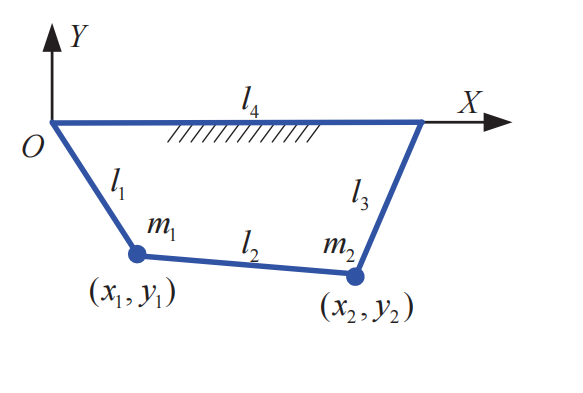
\includegraphics[width=0.6\textwidth]{Figure/双质点四连杆.png}
    }{
        \fbox{\parbox{0.5\textwidth}{\centering\vspace{3cm}%
        \textbf{[图片待插入]}\\[4pt] 双质点四连杆示意图\\[4pt]\vspace{3cm}}}
    }
    \caption{双质点四连杆}
    \label{fig:four_bar}
\end{figure}

广义坐标选为
\begin{equation}
    \bm{q} = \begin{bmatrix} x_1 & y_1 & x_2 & y_2 \end{bmatrix}^{\mathrm{T}}.
    \label{eq:four_bar_q}
\end{equation}

\paragraph{质点单摆}

\begin{figure}[H]
    \centering
    \IfFileExists{Figure/质点单摆.png}{
        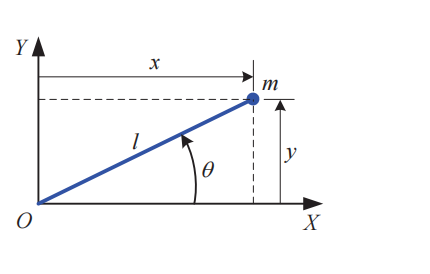
\includegraphics[width=0.5\textwidth]{Figure/质点单摆.png}
    }{
        \fbox{\parbox{0.4\textwidth}{\centering\vspace{3cm}%
        \textbf{[图片待插入]}\\[4pt] 质点单摆示意图\\[4pt]\vspace{3cm}}}
    }
    \caption{质点单摆}
    \label{fig:pendulum}
\end{figure}

广义坐标选为
\begin{align*}
    \bm{q} &= [\theta]; \\
    \bm{q} &= \begin{bmatrix} x & y \end{bmatrix}^{\mathrm{T}}.
\end{align*}

\paragraph{质点双摆}

\begin{figure}[H]
    \centering
    \IfFileExists{Figure/质点双摆.png}{
        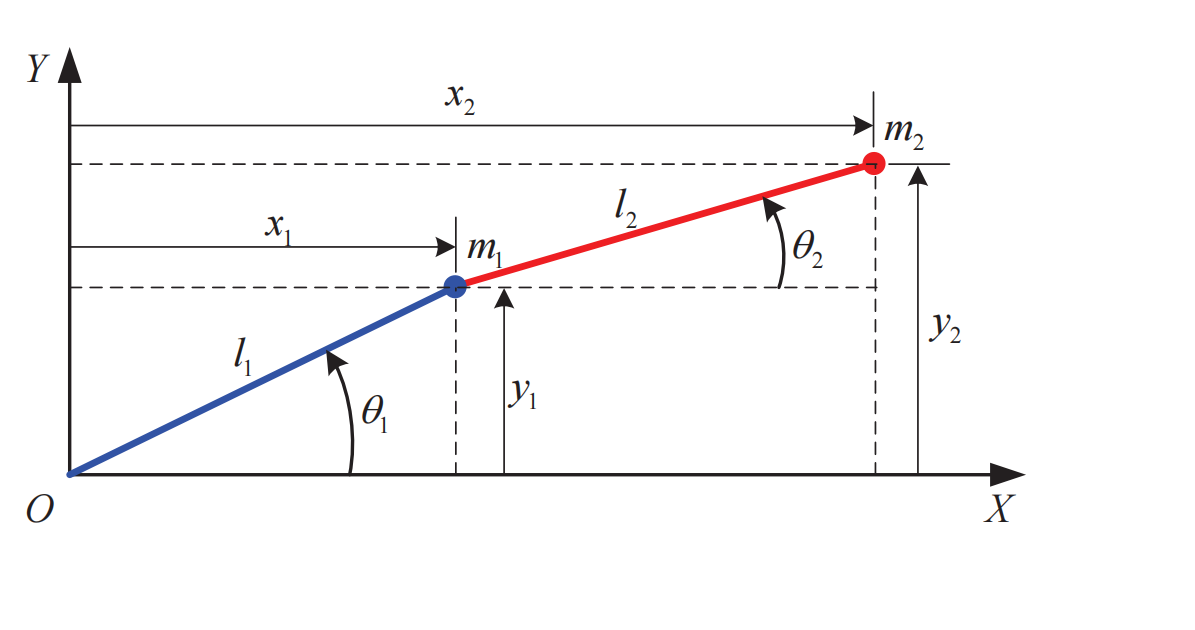
\includegraphics[width=0.65\textwidth]{Figure/质点双摆.png}
    }{
        \fbox{\parbox{0.55\textwidth}{\centering\vspace{3cm}%
        \textbf{[图片待插入]}\\[4pt] 质点双摆示意图\\[4pt]\vspace{3cm}}}
    }
    \caption{质点双摆}
    \label{fig:double_pendulum}
\end{figure}

广义坐标选为
\begin{align*}
    \bm{q} &= \begin{bmatrix} \theta_1 & \theta_2 \end{bmatrix}^{\mathrm{T}}; \\
    \bm{q} &= \begin{bmatrix} x_1 & y_1 & x_2 & y_2 \end{bmatrix}^{\mathrm{T}}.
\end{align*}
